\subsection{Thread scheduler}
As mentioned earlier, our scheduler implements User-Level Thread (UTL). The
user specifies the number of workers which are implemented with POSIX thread
and pinned to a specific core. The context-switching mechanism is similar to
that of Argobots and Boost coroutines, we make use of \texttt{fcontext}. The
idea is to maintains a separate stack for each thread. A few registers
(including the program counter) is saved and restored from an allocated space
in the stack. Morever, the context-switching is designed to not involve
Operating System (OS) system call, thus by-passing kernel code. This overall
reduces the latency of switching to a new context to less than a hundred
cycles.

Rather than designing a general purpose ULT, we focus on the two most important
operations for synchronization purpose: \texttt{ThreadWait} and
\texttt{ThreadSignal}. A possible implementation is \textit{condition
variable}. This is the typical mechanism in POSIX thread, and other ULT
library.  Condition variable is a generic container which can
be used as a building block for many other synchronization primitives. However,
it is still expensive as in general it requires a mutex lock and some queue
traversal when many threads are blocking.  An alternative is to use a
busy-waiting synchronization flag which has lower latency. However this is
considered even worst for scaling since the processor spends useless time
polling. Qthreads implements a slight modification notion of condition variable
namely \textit{full-empty bit}. However, internally each object is a waiting
queue and rescheduling requires expensive traveral of this queue to find
runnable threads and insert back to run queues.

Our thread scheduler targets a constant time overhead for both afortmentioned
operation. Marking a thread as runnable or waiting is only a single x86
instruction. The idea behind our thread scheduler is a novel use of bit-vector.
Rather than using a queue to implement a set of runnable thread, each bit in
the bit-vector indicates a schedulable thread. When a worker is created, it is
given a unique worker id, denotes as $\omega$.  When a thread is created by a
worker, it is assigned an unique id $\Gamma$ within the range of $[0,M-1]$, for
$M$ is the maximum concurrent threads for that worker.  For example, using a
vector of $8$ 64-bit words, we allow up to $512$ concurrent threads per worker.
A pair $(\omega, \Gamma)$ uniquely defines a thread in the system at a point in
time. During thread's creation time, the associated $\Gamma$ bit in its
bitvector structure is marked so that when the worker is free it will attempt
to schedule that thread to run. Algorithms \ref{algo:thread} further describes
our scheduling algorithms. 

\begin{algorithm}
  \caption{Thread scheduler}
  \label{algo:thread}
  \begin{algorithmic}[1]
    \Procedure{Scheduling}{$\omega$, V} \Comment{worker, bit-vector}
    \While {!$\omega$.stop} \Comment{loop until user ask to stop}
      \For{word in V}
      \If{word $\ne$ 0}
        \State localWord = 0
        \State AtomicExchg(word, localWord)
        \While {localWord64 $> 0$}
          \State b = FindFirstSet(localWord)
          \State localWord = FlipBit(localWord, b)
          \State ContextSwitch($b$)
        \EndWhile
      \EndIf
      \EndFor
    \EndWhile
    \EndProcedure
  \end{algorithmic}
\end{algorithm}

\begin{algorithm}
  \caption{Thread Operations}
  \label{algo:thread-ops}
  \begin{algorithmic}[1]
    \Procedure{ThreadWait}{}
      \State ContextSwitch($\omega$)
    \EndProcedure
    \\ 
    \Procedure{ThreadSignal}{sync}
      \State AtomicBitSet(sync.$\omega$.V, sync.$\Gamma$)
    \EndProcedure
  \end{algorithmic}
\end{algorithm}

The scheduler works at 64-threads granularity instead of 1-thread traditionally.
By using an atomic exchange instruction to swap the interested word to local variable, we
are able to continously perform read/write from/to this variable without
accessing the main memory. This is not only ensures progress property for all
threads because we can schedule them in order, it solves the problem of having
no atomic read-modify-write instructions operating at bit level.

Algorithms \ref{algo:thread-ops} describes the two thread operations.
\texttt{ThreadWait} simply switch back to the worker scheduler based on current
worker id (i.e. $\omega$) On the other hand, \texttt{ThreadSignal} shall access
the bit-vector and atomically set the bit in the appropriate word based on the
the same information stored in the synchronization object. $\omega$ and
$\Gamma$ are stored in thread local-storage of the worker, and is updated
whenever a new context is switch to.

There are couple of issues worth discussing on the above design.  Firstly, note
that \texttt{ThreadWait} is executed in the same kernel thread as the thread
scheduler associating with the running ULT while \texttt{ThreadSignal} can be
executed anywhere. Thus, It is errornous to perform \texttt{ThreadSignal}
multiple times on the same object since they will be treated as one or more
signal depending on the time the worker looks at the bit-vector. It is also
erronous to \texttt{ThreadWait} when the associted \texttt{ThreadSignal} has
been performed. In practise for each MPI request we use an additional flag to
indicate whether the signal has been executed before performing the
\texttt{ThreadWait}. This is important for non-blocking communication in the
case of \texttt{MPI_Waitall} since the communication can be completed before
the thread attempts to wait.

The next issue is that the performance shall degrades when we increase the
maximum number of threads since iterating over the bit-vector word by word is
more expensive. We tackle this issue by using a hierachical design of
bit-vector.  That is, we could use an additional bit-vector as a hint to index
into the original bit-vector. Specifically, each bit in the secondary
bit-vector indicates which word in the first level may have a schedulable
thread. More specifically, \texttt{ThreadSignal} will perform a bit set first
into the first level then a bit set into the second level. The scheduler will
first look into the second level to find a potential word and go directly to
that word to look for schedulable threads. %Recall that the secondary bit-vector
%is shared among a group of threads, thus It can happen that the secondary might
%indicate the thread is schedulable, but when it arrives at the first level the
%thread is already scheduled. However, this situation does not affect the
%correctness since the thread will not be scheduled twice in any situation.
Using this scheme, suppose we use one word for the secondary level bit-vector,
each bit represents a 64-bit word in the first level, then each worker can
support up to $4096$ threads. And since eight words can fit in a cache line and
better to read together, we can use 1 bit to represent a set of eight 64-bit.
Similarly by having eight words in the secondary level we can support $262144$
concurrent threads per worker. With a small number of worker, we can go up to
our goal of million thread without sacrifying much performance. Also note that
this is the maximum number of concurrent threads; when a thread completes its
current task, it can be re-used for launching another task.

There is an fairness issue with the thread scheduler i.e. thread with lower
index typically is scheduled before thread with higher index. There are a few
solutions to improve fairness for example occasionally traverse the bit-vector
in different orders. We however currently ignore this problem and leave it for
future works. Having said that, this issue is not severe since our algorithms
still ensure progress property. If a thread is marked as schedulable, it's
eventually will be scheduled in a bounded number of steps. To show that this is
true, consider the atomic exchange as taking a snapshot of the global state. In
this snapshot, if a thread is marked it will be scheduled after all threads
having smaller index are scheduled, which is bounded by the maxmimum number of
allowed concurrent threads $M$.

\subsection{Concurrent Hash-Table}
Our concurrent hash-table is not deviated very much from conventional
concurrent hash-table. We however find opportunity to optimize further by taking 
advantage of some semantics requirement that we have mentioned.

Firstly, we use a spinlock per bucket. This is an viable option since we could
control the table size to reduce the hash collision to minimal. The table size is
related directly to how many concurrent operations which is controlled by 
our packet pool size. When there is no collision, the conflict can only happen
between communication server and a thread when both try to insert into the same
bucket at the same time. With a small number of conflicts, a spinlock is
sufficient for synchronization and allow a very simple design.

Secondly, we design each bucket as an 4-entry array. Each entry consists of two
64-bit words. Within each 4-entry, one entry will be used as \textit{control
entry} and the other three are used for \textit{data entry}. The control entry
has an atomic flag for spin locking, and a pointer to point to the next 4-entry
bucket in case we have more than 3 collisions. A data entry consists of two
64-bit words of key and value pair. In total, 4-entry takes 64-bytes and
typically fits in a cache line. Thus we suffer only 1 cache miss when trying to
lock the bucket and the data can be read without more cache misses.

Lastly, the \texttt{insert} operation also returns the address of the
associated entry having the key in memory. This allows the \texttt{empty}
operation to be a single instruction/single memory write to set the value
associated with key to $\bot$. This is only possible when only one thread can
write to an entry key which is true when no concurrent communication with the
same tag is allowed.

In conclusion, with the above optimization, the \texttt{empty} operation is
lock-free and wait-free, costs only 1 memory write. The \texttt{insert}
operation is cache-friendly and is typically wait-free, costs also 1 memory
write in the common case of no hash collision (write is made to spin-lock;
other accesses are in cache).

\subsection{Concurrent Packet Pool}
In general, the packet pool can be implemented using a lockfree stack. A pool
\texttt{free} is translated to a stack \texttt{push}, and \texttt{alloc} is
translated to a stack \texttt{pop}. At the initialization, a fixed number of
packet is initialized from the main memory and \texttt{push} to the container.
The Last-In-First-Out (LIFO) property allows good temporal locality for
writing/reading to/from the content of a data packet. In a single-threaded
environment this design is sufficient for good performance, but not for the
case of multi-core/multi-threaded. Consider a packet recently being used by a thread
and returned to the pool, this packet could be subsequently obtained by a different thread
running in a different core. This leads to several cache misses since the cacheline
is momently owned by the first thread. An example is when two threads running in 
two different cores alternatively perform \texttt{MPI_Send}.

\begin{figure}[t]
  \centering 
  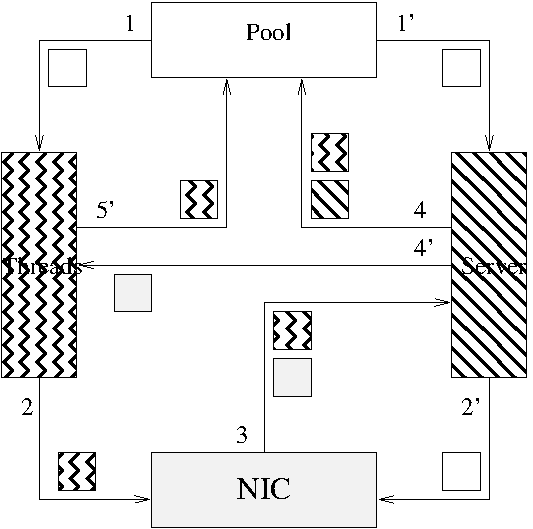
\includegraphics[width=0.3\textwidth]{fig/packetlife.pdf}
  \caption{Packet life cycle: (1) A thread sending data obtain a packet from the
    pool; (2) The thread writes data into the packet and submit it to the NIC;
    (1', 2') Communication server obtains a packet for receiving data
    and posts the packet to the NIC;
    (3) The server polls the NIC and obtains the packet back (either send/recv packet).
    (4) If the packet is for sending, it is returned to the pool;
    If the packet is for receiving and there is a request, the server copies the data
    and returns the packet to the pool;
    (4') If the packet is for receiving and the there is no request, the packet is inserted to hash-table.
    (5') The thread takes packet from the hash-table copies the data before returning it back to the pool.}
  
  \label{fig:packetlife}
\end{figure}

Figure \ref{fig:packetlife} explains how different components in our system
might change the affinity of data inside a packet. The figure shows the life of
a packet from the time it leaves the pool until it is returned. As explained in
the figure, when a packet returns to the pool, it can only has the affinity
of either the communication server or one of the worker thread. More specifically,
if the packet is used for sending data, it shall have the locality of the thread;
if the packet is used for receiving data, it shall have the locality of either
the thread or the server depending on whether the associated request and the
packet is received first. Moreover, when the packet is posted by the server
to the NIC for receiving data, the packet shall lose any affinity it has since
the NIC will perform a write over the packet.

Analysing the packet life cycle motivates us a new design for the packet pool.
We split the centralized packet management into a private pool per worker and a
shared pool per communication worker. Initially, there is a fixed number of
packets for each of the pool. At runtime, we design an algorithms to allow
moving packets among those pool depending on their usages.  Our goal is to
maintain good locality per hardware thread but does not block if there is
available resources.

The private pool consists of packets that are identified as having affinity of
the associated hardware thread. It is implemented as a fixed size double-ended
queue (deque). The deque has three main operations: \texttt{popTop},
\texttt{pushTop}, and \texttt{popBottom} which allows LIFO accessing at the top
of the queue, and also allows poping from its bottom. The idea is that at the
bottom of the deque are packets that are least recently used and are better
candidates for other purposes. That is, when the private pool is full, it
performs \texttt{popBottom} and pushed back to the shared pool.

When a packet for sending is needed by a thread, a \texttt{popTop} is performed
with the private pool of the current worker, which guarantees giving the last
packet that was read or written by the same worker. If the private pool is
empty, the shared pool is accessed for extra packets.  Alternatively, when a
packet is needed for receiving data by the communication server, the server
first try to obtains packets from its shared pool. If the shared pool is empty,
the server now performs a \textit{steal} by randomly chosing a private pool and
perform the \texttt{popBottom} operation.

The private pools can be thought as caches, and the shared pool can be thought
as the main memory. When ``the cache'' is full, it evicts the least recently
used to the ``main memory''. Our heuristic essentially performs
resource-balancing among the set of packets by moving it around pools with the
locality taken into account. Since the private pool is only shared between a
worker thread and the communication server, currently we implemented it using a
simple fixed-size buffer with a spinlock. The shared pool is accessed by more
than two threads, thus implemented using a lock-free stack.
